%%%%%%%%%%%%%%%%%%%%%%%%%%%%%%%%%%%%%%%%%%%%%%%%%%%%%%%%%%%%%%%%%%%%%%%%%%%%%%%%%%%%%%%%%%
%                                     SETTINGS                                           %
%%%%%%%%%%%%%%%%%%%%%%%%%%%%%%%%%%%%%%%%%%%%%%%%%%%%%%%%%%%%%%%%%%%%%%%%%%%%%%%%%%%%%%%%%%
\documentclass[aspectratio=169]{beamer}


\usepackage{amsmath,amssymb}
\usepackage{graphicx}
\usepackage{subcaption}
\usepackage{standalone}
\usepackage[makeroom]{cancel}
\usepackage{appendixnumberbeamer}
\usepackage{hyperref}
\usepackage{booktabs}
\usepackage{xcolor}
\usepackage{units}

\usetheme{Montpellier}

\setbeamertemplate{itemize items}[circle]
\setbeamertemplate{footline}[frame number]
\setbeamertemplate{navigation symbols}{}

\usepackage[backend = bibtex,
			style = authoryear,
			maxnames = 5,
			maxcitenames = 3,
			doi = false,
			eprint = false]{biblatex}
\addbibresource{../biblio.bib}

\newcommand{\aref}[1]{\hyperref[#1]{Appendix~\ref{#1}}}
\newcommand{\themename}{\textbf{\textsc{metropolis}}\xspace}
\newcommand\Fontsmall{\fontsize{8}{7.2}\selectfont}

\AtBeginSection[]{
	\begin{frame}
		\vfill
		\centering
		\begin{beamercolorbox}[sep=8pt,center,shadow=true,rounded=true]{title}
			\usebeamerfont{title}\insertsectionhead\par%
		\end{beamercolorbox}
		\vfill
	\end{frame}
}

%\AtBeginSection[]{  % Add slide with content before each section
%	\begin{frame}
%		\frametitle{Outline}
%		\tableofcontents[currentsection]
%\end{frame}}

%%%%%%%%%%%%%%%%%%%%%%%%%%%%%%%%%%%%%%%%%%%%%%%%%%%%%%%%%%%%%%%%%%%%%%%%%%%%%%%%%%%%%%%%%%
%                                     TITLE                                              %
%%%%%%%%%%%%%%%%%%%%%%%%%%%%%%%%%%%%%%%%%%%%%%%%%%%%%%%%%%%%%%%%%%%%%%%%%%%%%%%%%%%%%%%%%%
\title{Do Minimum Wages Increase Rents?}
\subtitle{Evidence from US ZIP Codes Using High-Frequency Data}
\date{\today}
%\date{}
\author{Gabriele Borg \and Diego Gentile Passaro \and Santiago Hermo}
\institute{Brown University}
% \titlegraphic{\hfill\includegraphics[height=1.5cm]{logo.pdf}}

%%%%%%%%%%%%%%%%%%%%%%%%%%%%%%%%%%%%%%%%%%%%%%%%%%%%%%%%%%%%%%%%%%%%%%%%%%%%%%%%%%%%%%%%%%
%                                         BODY                                           %
%%%%%%%%%%%%%%%%%%%%%%%%%%%%%%%%%%%%%%%%%%%%%%%%%%%%%%%%%%%%%%%%%%%%%%%%%%%%%%%%%%%%%%%%%%
\begin{document}
\maketitle


%%% Introduction %%%
	
\begin{frame}
	\frametitle{Motivation}
	
	Research on minimum wage (MW) has mostly focused on employment.
	% States: people work and reside under same MW.
	
	\vspace{1.5mm}
	However, MW policies are \textit{place-based}, so one should expect broader effects 
	in the local economy:
	\begin{enumerate}[$\Rightarrow$]
		\item Housing market.
	\end{enumerate}

	\pause
	\vspace{3mm}
	Because
	\begin{itemize}
		\vspace{.5mm} \item people tend to work and reside in different locations; and 
		%\parencite{MonteEtAl2018}
		\vspace{.5mm} \item MW levels tend to vary within metropolitan areas;
		%\parencite{DubeLindner2021}
	\end{itemize}
	% MonteEtAl2018: Change in the distribution of share who work in same county
	% DubeLindner2021: 42 local MWs in the US
	\vspace{.5mm} 
	accurate welfare analysis of MW increases requires understanding the consequences of 
	the spatial re-distribution of income they induce.
	%% People tend to live and work under different MW levels!
	
	%A canonical version of the monocentric city model suggests that wage increases will 
	%fully pass-through to rents.
\end{frame}

\begin{frame}
	\frametitle{This paper}
	We investigate the effect of MW policies on rents between Jan 2010 and Dec 
	2019:
	\begin{itemize}
		\vspace{.5mm} \item Estimate elasticity of median rents to workplace and 
		residence MWs;
		
		\vspace{.5mm} \item Estimate pass-trough of MW increases to rents.
	\end{itemize}
	
	\vspace{3mm}
	\pause
	To do so, we:
	\begin{itemize}
    	\vspace{.5mm} \item Exploit high-frequency rents data from Zillow at a fine 
    	geography (ZIP code);
    	
    	\vspace{.5mm} \item Propose a novel measure of exposure to MW changes based on 
    	commuting shares;
    	
    	\vspace{.5mm} \item Leverage variation in MW levels \textit{within} metropolitan 
    	areas to estimate effect of workplace and residence MWs changes.
	\end{itemize}
\end{frame}

\begin{frame}
	\frametitle{Preview of Findings}
	
	We find that:
	\begin{itemize}
		\vspace{.5mm} \item
		The elasticity of rents to workplace MW is 0.072--0.108;
		% Controlling for residence MW
		
		\vspace{.5mm} \item
		If residence MW also increases, the elasticity is 0.034--0.061;
		% Controlling for residence MW
		
		\vspace{.5mm} \item
		Failing to account for commuting patterns results in an elasticity of 
		0.026--0.058 \textit{only at residence};
		
		\vspace{.5mm} \item
		The pass-through of MW to rents is at least 22\%.
	\end{itemize}
	
	\pause
	\vspace{4mm}
	Overall, our results highlight the importance of accounting for variation of MWs 
	within metropolitan areas and commuting patterns of workers when evaluating MW 
	policies.
\end{frame}


%\begin{frame}
%	\frametitle{Literature}
%	
%	Botija.
%	
%\end{frame}


%%% Outline %%%
\begin{frame}
	\frametitle{Outline}
	\tableofcontents[hideallsubsections]
\end{frame}

%%% Main body %%%
\section{A Partial Equilibrium Model of the Rental Market}
	
\subsection{Overview}
\begin{frame}
	\frametitle{Overview}
	
	Goals of the model:
	\begin{itemize}
		\item Motivate a new MW measure: the experienced MW.
		\item Motivate our empirical strategy: use commuting patterns to account for 
		spillovers of MW policies.
	\end{itemize}
	
	\pause
	\vspace{2mm}
	The model is \textit{not} intended to:
	\begin{itemize}
		\item Describe within-city residential sorting or local goods markets.
		\item Perform welfare analysis of MW policies.
	\end{itemize}

\end{frame}

%%: Let me show a simple example that illustrates the workings of the model

\begin{frame}
	\frametitle{Simple Illustration}
	
	No commuting across ZIP codes:
	\input{../input/example_1}
	
	\pause
	\vspace{2mm}
	All residents of A work in B and vice-versa:
	\input{../input/example_2}
	
\end{frame}

\subsection{Set-up}
\begin{frame}
	\frametitle{Set-up}
	
	%% Intuition: workers get income, eat tradable good with exogenous price, and then
	%% decide to consumer local good and housing.
	%% ==> We model the housing market
	
	\begin{itemize}
		\item $\mathbb{Z}$: set of ZIP codes, indexed by $i$ (residence) and $z$ 
		(workplace).
		
		\pause
		\vspace{2mm}
		\item $L_{i z}$: measure of workers who reside in $i$ and work in $z$.
		\begin{itemize}
			\item Total measure of workers $\mathcal{L}=\sum_{i \in \mathbb{Z}} 
			\sum_{z \in \mathbb{Z}} L_{i z} $ is assumed exogenous.
		\end{itemize}
	
		\pause
		\vspace{2mm}
		\item $y_{i z} = y_{i z} \left(\underline{w}_i, \underline{w}_z\right)$: 
		disposable income, where:
		\begin{itemize}
			\item $\underline{w}_i$ and $\underline{w}_z$ are residence and 
			workplace MWs.
		\end{itemize}
	
		\pause
		\vspace{2mm}
		\item $H_{i z} \left(r_i, y_{i z} \right)$: housing demand, where $r_i$ 
		represents housing rents.
		
		\pause
		\vspace{2mm}
		\item $D_i \left(r_i \right)$: housing supply.
	\end{itemize}
	
\end{frame}


\begin{frame}
	\frametitle{Assumptions}
	
	Disposable income $y_{i z}$:
	\begin{itemize} \small
		\item decreasing in residence MW, $\frac{d y_{i z}}{d \underline{w}_i} < 0$.
		
		\vspace{.5mm}
		\item increasing in workplace MW, $\frac{d y_{i z}}{d \underline{w}_z} > 0$.
	\end{itemize}

	\pause
	\vspace{2mm}
	Housing demand $H_{i z} \left(r_i, y_{i z} \right)$:
	\begin{itemize} \small
		\item decreasing in rents, $\frac{d H_{i z}}{d r_i} < 0$;
		
		\vspace{.5mm}
		\item increasing in disposable income, $\frac{d H_{i z}}{d y_{i z}} > 0$.
	\end{itemize}
	
	\pause
	\vspace{2mm}
	Housing supply: 
	\begin{itemize} \small
		\item $D_i \left(r_i \right)$ is increasing in rents, $\frac{d D_i}{d 
			r_i} > 0$.
	\end{itemize}
\end{frame}

\subsection{Equilibrium and Comparative Statics}
\begin{frame}
	\frametitle{Equilibrium}
	
	The rental market of ZIP code $i$ is in equilibrium if
	
	$$ \sum_{z\in\mathbb{Z}} L_{i z} H_{i z} (r_i, y_{i z}) =  D_i (r_i) .$$
	
	We denote equilibrium rents as $r^*_i = f\left( 
	\{\underline{w}_j\}_{j\in\mathbb{Z}} \right)$. 
	%% A function of MWs in the entire metropolitan area.
	
	% As lhs is decreasing and rhs is increasing, curves cross only once.
	% To guarantee r^*_i > 0, assume D_i(r_i = 0) is high enough
	
	\vspace{5mm}
	\pause
	We are interested in the effects of MW policies on rents.
	\vspace{1mm}
	\begin{itemize} \small
		\item What are the consequences of not accounting for both residence and 
		workplace MWs?
		\vspace{.5mm}
		\item Under what conditions one can reduce the dimensionality in the rents 
		function?
	\end{itemize}

\end{frame}


\begin{frame}
	\frametitle{The Differential Effect of Residence and Workplace MWs}
	
	\small
	\textbf{Proposition 1:} \textit{Consider a new MW policy. Under the assumptions of
	\begin{itemize}
		\item fixed distribution of workers across residence and workplace locations;
		\pause
		\item disposable income is increasing in workplace MW and decreasing in residence 
		MW;
	\end{itemize}
	\pause
	we have that workplace-MW hikes \textbf{increase} rents, and residence-MW hikes, 
	\textbf{conditional} on workplace MWs, \textbf{decrease} rents.}
	
	\pause
	\vspace{1.5mm}
	\textit{Furthermore, assuming that
		\begin{itemize} 
			\item elasticities of rents to income and of income to MWs do not vary by 
			workplace;
		\end{itemize}
	\pause
	we can write the change in \textbf{log rents} as a function of the change in two 
	MW-based measures: \textbf{experienced log MW} and \textbf{statutory log MW}.}
	
\end{frame}

\begin{frame}[label = proof_main]
	\frametitle{Proof of Proposition 1}
	
	%% Joke: mention Simon and Blume
	First part of the proposition can be shown applying implicit function theorem. 
	\hyperlink{proof_prop_1}{\beamerbutton{Details}}
	
	\pause
	\vspace{2mm}
	As for the second part, we can write
	
	$$
	d \ln r_i
	= \underbrace{\frac{\xi_i^y \epsilon_i^z}
		   {\eta_i - \sum_z \pi_{i z} \xi_{i z}^r}}_{\beta_i > 0}
		   \underbrace{\sum_z \pi_{i z} d \ln \underline{w}_z}_{
		   		\substack{\text{Exp. log MW}\\\text{at residence}}}
	+ \underbrace{\frac{\xi_i^y \epsilon_i^i}
		   {\eta_i - \sum_z\pi_{i z}\xi_{i z}^r}}_{\gamma_i < 0}
		   \underbrace{d \ln \underline{w}_i}_{
		   		\substack{\text{Stat. log MW}\\\text{at residence}}}
	$$
	
	\vspace{-1mm}
	where 
	\begin{itemize} \small
		\item $\pi_{i z}$: \textit{share} of $i$'s residents 
		working in $z$;
		
		\item $\xi_{i z}^r$ and $\xi_{i}^y$: 
		elasticities of $H_{i z}$ wrt $r$ and $y$ 
		($\xi_{i}^y$ assumed constant over $z$);
		%%% evaluated at average housing demand in ZIP code;
		
		\item $\epsilon_{i}^i$ and $\epsilon_{i}^z$: elasticities of 
		$y_{i z}$ wrt $\underline{w}_i$ and $\underline{w}_z$
		(both assumed constant over $z$);
		
		\item $\eta_i$: elasticity of \textit{housing supply}.
	\end{itemize}
	
\end{frame}

\begin{frame}
	\frametitle{Implications of the Model}
	
	Per equation above, we are interested in the parameters
	$$ \beta_i = \frac{\xi_i^y \epsilon_i^z}
	{\eta_i - \sum_z \pi_{i z} \xi_{i z}^r} > 0 
	\quad \quad \quad 
	\gamma_i = \frac{\xi_i^y \epsilon_i^i}
	{\eta_i - \sum_z\pi_{i z}\xi_{i z}^r} < 0 .	$$
	
	%% Empirical model gets to average beta. Mention heterogeneity
	%% Also mention importance of gamma for distributional consequences of MW changes
	
	\vspace{3mm}
	\pause
	Imagine an econometrician who omits one of the measures in the above model:
	\begin{itemize}
		\item It can be shown that the resulting elasticity will be between $\gamma_i$ 
		and $\beta_i$.
	\end{itemize}
\end{frame}

\subsection{Discussion}
\begin{frame}
	\frametitle{Discussion}
	
	\begin{itemize}
		\item Including both the statutory and experienced log MW should allow estimation 
		of the differential effect of MWs on rents from workplace and residence changes.
		\vspace{1mm}
		\begin{itemize}
			\item Assumption of fixed $\pi_{i z}$ shares appears plausible in short-run.
			
			{\color{gray} \footnotesize \parencite{MonteEtAl2018, CegnizEtAl2019, 
			PerezPerez2020}} 
			% MonteEtAl2018 studies the shift in distribution of residence workplace at 
			%%%   the decadal level // Use "share who work in same county"
			% PerezPerez2020 finds no effect of MWs on resident shares and low effect on 
			%%%   employment shares // Model at level of counties
			
			\vspace{1mm}
			\item Assumption that local MWs decrease disposable income is consistent with 
			literature on price effects of MWs.
			
			{\color{gray} \footnotesize \parencite{Allegretto2018, Leung2020}}
			% Allegretto2018 on restaurants following MW hike in San Jose, CA, in 2013
			% Leung2020 effect of MW on supermarkets (Nielsen data)
		\end{itemize}
		
		\vspace{2.5mm}
		\item Can test the model's rationale by including only the statutory or 
		experienced log MW in empirical models and comparing with main estimates.
	\end{itemize}
	
\end{frame}



\section{Data and Sample}
	
\subsection{Zillow}

\begin{frame}[label = zillow]
	\frametitle{Zillow Data}
	
	\begin{itemize}
		\item Leader online real estate and rental platform in the U.S. {\small (more 
		than 110 million homes and 170 million unique monthly users in 2019).}
		
		\vspace{2mm} \item
		Provides \textit{median} rents data at ZIP code, county, and state levels 
		at a monthly frequency for several housing categories.
		
		\pause
		\vspace{2mm} \item
		Use category single-family, condominium, and cooperative houses (SFCC):
		\begin{itemize}
			\item Most common housing type in the U.S.
			\item Most populated series in Zillow.
			%%\item Captures trends in metropolitan housing markets. 
			%%\hyperlink{zillow_safmr}{\beamerbutton{Comparison SAFMR}}
		\end{itemize}
		
		\pause
		\vspace{2mm} \item
		Limitation: Zillow sample is not random.
	\end{itemize}
\end{frame}

\begin{frame}[label = zipcodes_map]
	\frametitle{Comparison between Zillow Sample and Population Density}
	
	\vspace{-1mm}
	\begin{figure}
		\begin{subfigure}[t]{.49\textwidth}\centering
			\includegraphics[width = .92\textwidth]
				{../../analysis/descriptive_maps/output/sample_map.png}
		\end{subfigure}
		\begin{subfigure}[t]{.49\textwidth}\centering
			\includegraphics[width = .92\textwidth]
				{../../analysis/descriptive_maps/output/popurban_density_map.png}
		\end{subfigure}
		\begin{minipage}{.95\textwidth} \scriptsize	\vspace{1mm} 
			\textit{Notes}: Left panel shows ZIP codes available in Zillow data. Right 
			panel shows the urban population density for the top 100 metropolitan areas 
			in the U.S. from the 2008-2011 ACS (winsorized at the 99th percentile).
		\end{minipage}
	\end{figure}

	\hyperlink{tab_comparison}{\beamerbutton{Comparison Table}}

\end{frame}

% Should we add something about Zillow vs SAFMR? 

\subsection{Minimum Wages}

\begin{frame}[label=stat_MW]
	\frametitle{The Statutory MW}
	
	\begin{itemize}
		\item
		Collect MW data at state, county and city levels between Jan 2010 and Dec 2019.
		
		\vspace{2mm} \item
		Assign those data to ZIP codes.
		
		\vspace{2mm} \item
		Define statutory MW in ZIP code as maximum between state and local levels.
		
		\pause
		\vspace{2mm} \item
		ZIP codes available in Zillow contain 18,689 changes at the ZIP code-month level.
		\vspace{-3.5mm} 
		\begin{itemize} \small
			\item 151 state-level changes.
			\item 182 county- and city-level changes.
		\end{itemize}
		%% We use 4,224 events at the ZIP code-month level in our estimating panel
		
		\hyperlink{dist_mw_changes}{\beamerbutton{Distribution of MW changes}}
	\end{itemize}
	
\end{frame}

\begin{frame}
	\frametitle{Using LODES to construct the experienced log MW}
	
	Construct \textbf{origin-destination matrix} at ZIP code level from 2017 LODES.
	%% Original data comes at the block-group level
	Observe:
	\begin{itemize} \small
		\item Number of workers residing in a ZIP code and working in every other 
		ZIP code.
		\item Analogously, number of workers younger than 29 and earning less than 
		\$1,251.
		%% Exp MW constructed using any of these measures gives similar results
	\end{itemize}
	
	\pause
	\vspace{2.5mm}
	Define \textbf{experienced log MW} in ZIP code $i$ month $t$ as
	$$
	\underline{w}^{\text{exp}}_{it} = 
	\sum_{z \in \mathbb{Z}_i} \pi_{i z} \ln \underline{w}_{zt} \ ,
	$$
	%% IMPORTANT: We average the log of the MW! (Not log the average)
	\vspace{-2.5mm}
	where
	\vspace{1mm}
	\begin{itemize} \small
		\item $\mathbb{Z}_i$ are workplace locations of $i$'s residents, and
		\item $\pi_{i z} = \frac{L_{i z}}{L_i}$ is the share of $i$'s residents who work 
		in $z$.
	\end{itemize}
\end{frame}

\begin{frame}[label=san_diego_mw]
	\frametitle{The California MW Increase of January 2019 in San Diego} 
	
	%% San Diego MW Dec 2019: $11.5
	%% California MW Dec 2019: $11 (for large employers)
	%% Level MW Jan 2020 in both places: $12
	
	\begin{figure}
		\begin{subfigure}[b]{0.49\textwidth}
			\includegraphics[width = .85\textwidth]
				{../../analysis/descriptive_maps/output/San_Diego_mw_msa.png}
		\end{subfigure}%
		\begin{subfigure}[b]{0.49\textwidth}
			\includegraphics[width = .85\textwidth]
				{../../analysis/descriptive_maps/output/San_Diego_expmw_msa.png}
		\end{subfigure}
	\end{figure}
	
	\hyperlink{san_diego_rents}{\beamerbutton{Map rents}}
\end{frame}

\subsection{Sample Selection}

\begin{frame}[label=san_diego_mw]
	\frametitle{Other Data Sources and Sample Selection} 
	
	Other data sources:
	\begin{itemize}
		\item Economic controls from the Quarterly Census of Employment and Wages 
		{\small (QCEW)}.
	\end{itemize}
	
	\pause
	\vspace{3mm}
	ZIP codes enter Zillow data in different months.
	\begin{itemize} \small
		\item To account for composition changes in the sample, we use ZIP codes with 
		valid rents data as of July 2015 as baseline. (1,305 ZIP codes, 4,224 events.)
	\end{itemize}
	
	\vspace{2.5mm}
	We conduct several exercises changing the sample, and find consistent results.
%	\begin{itemize} \small
%		\item Use all ZIP codes available controlling for ``cohort $\times$ time-period'' 
%		fixed effects.
%		\item Use fully balanced panel starting from July 2015.
%		\item Weight regression to match key moments in the distribution of ZIP codes of 
%		top 100 CBSA.
%	\end{itemize}
	% Results are similar. Won't show everything for interest of time.
	
\end{frame}

\begin{frame}[label=san_diego_mw]
	\frametitle{Baseline Sample: Summary Statistics} 
	
	\begin{table}
		\scalebox{.87}{
% Table created by stargazer v.5.2.2 by Marek Hlavac, Harvard University. E-mail: hlavac at fas.harvard.edu
% Date and time: Fri, Dec 11, 2020 - 1:50:17 PM
\begin{tabular}{@{\extracolsep{5pt}}lccccc} 
\\[-1.8ex]\hline 
\hline \\[-1.8ex] 
Statistic & \multicolumn{1}{c}{N} & \multicolumn{1}{c}{Mean} & \multicolumn{1}{c}{St. Dev.} & \multicolumn{1}{c}{Min} & \multicolumn{1}{c}{Max} \\ 
\hline \\[-1.8ex] 
Statutory MW & 155,295 & 8.08 & 1.21 & 7 & 16 \\ 
Experienced MW & 155,295 & 8.06 & 1.21 & 6.29 & 14.98 \\ 
Median rent psqft. SFCC & 113,375 & 1.27 & 0.83 & 0.47 & 7.25 \\ 
Median rent SFCC & 125,644 & 1,651.10 & 702.99 & 595.00 & 6,595.00 \\ 
Avg. wage Fin. activities & 151,032 & 1,561.71 & 961.88 & 0.00 & 9,557.00 \\ 
Employment Fin. activities & 151,032 & 59,595.23 & 75,840.23 & 0.00 & 397,839.00 \\ 
Estab. count Fin. activities & 151,032 & 5,105.58 & 5,201.89 & 31.00 & 30,405.00 \\ 
\hline \\[-1.8ex] 
\end{tabular} 
}
		\vspace{4mm}
		\begin{minipage}{0.95\textwidth} \scriptsize
			Notes: The table shows summary statistics of some variables in our baseline 
			estimating sample, which includes 1,305 ZIP codes and runs from January 2010 
			to December 2019.
		\end{minipage}
	\end{table}
\end{frame}


\section{Empirical Strategy}
	
\subsection{Empirical Models}

\subsection{Static Model}

\begin{frame}[label = stat_only_model]
	\frametitle{Static (statutory only) model}
	
	Ignoring the experienced MW, one may estimate the following first differences model:
	
	$$
	\Delta \ln r_{ict} = \tilde\delta_t + 
	\tilde\beta \Delta \ln \underline{w}_{ict} + 
	\Delta \mathbf{X}^{'}_{ict} \tilde\eta + 
	\Delta \tilde\varepsilon_{ict} ,
	$$
	
	where	
	\begin{itemize} \small
	\item ZIP code $i$, county $c$, month $t$;
	
	\item \vspace{1mm} $r_{ict}$: rents per square foot;
	
	\item \vspace{1mm} $\ln \underline{w}_{ict}$: statutory log MW;
	
	\item \vspace{1mm} $\tilde\delta_t$: month fixed effects (ZIP code FE $\tilde\alpha_i 
	$ is 
	implicit);
	
	\item \vspace{.5mm} $\mathbf{X}_{ict}$: time-varying controls.
	\end{itemize}
\end{frame}

\begin{frame}
	\frametitle{Static (statutory only) model: Identification assumption}
	
	For causal effect of the MW need conditional \textit{strict exogeneity}.
	
	\vspace{1.5mm}
	Formally, for every period $t$ need to assume:
	
	$$
	E \left[\Delta \tilde\varepsilon_{ict} \Delta \ln \underline{w}_{ic\tau}  
	\big| \tilde\delta_t, \Delta \mathbf{X}_{ict} \right] = 0
	\quad \quad \forall \tau \in \left[ \underline{T}, \overline{T} \right] .
	$$
	
	\pause
	\vspace{2mm}
	\textbf{In words}: conditional on FEs and controls, unobserved innovations to rent 
	shocks are uncorrelated with past and future values of log MW changes {\color{blue} 
	in same ZIP code}.
	
\end{frame}

\begin{frame}
	\frametitle{Static Model}
		
	Now add experienced MW:
	$$
	\Delta \ln r_{ict} = \delta_t +
	    \beta {\color{red}\Delta \underline{w}^{\text{exp}}_{ict}} +
		\gamma {\color{blue} \Delta \ln \underline{w}_{ict}} + 
		\Delta \mathbf{X}^{'}_{ict} \eta + 
		\Delta \varepsilon_{ict} ,
	$$
	
	where $\underline{w}^{\text{exp}}_{it}$ is experienced log MW {\small (Recall 
	$\Delta \underline{w}^{\text{exp}}_{it} = \sum_{z \in \mathbb{Z}_i} \pi_{i z} \Delta 
	\ln \underline{w}_{zt}$)}.

	\pause
	\vspace{2mm}
	For causal effect of $\beta$ we need:
	$$
	E \left[\Delta \varepsilon_{ict} {\color{red} \Delta 
	\underline{w}^{\text{exp}}_{ic\tau}} 
	\big| {\color{blue}\Delta \ln \underline{w}_{ict}}, \delta_t, \Delta 
	\mathbf{X}_{ict} \right] = 0
	\quad \quad \forall \tau \in \left[ \underline{T}, \overline{T} \right]
	$$
	
	\pause
	\vspace{2mm}
	\textbf{In words}: conditional on FEs, controls, and {\color{blue} MW in same ZIP 
	code}, unobserved innovations to rent shocks are uncorrelated with past and future 
	values of log MW changes {\color{red} in nearby ZIP codes}.
\end{frame}


\begin{frame}
	\frametitle{Static Model: Identification Assumption}
	
	Thus, for causal effect of $\beta$ we need:
	$$
	E \left[\Delta \varepsilon_{ict} \Delta \underline{w}^{\text{exp}}_{ict}  
	\big| \Delta \ln \underline{w}_{ict}, \delta_t, \Delta 
	\mathbf{X}_{ict} \right] = 0
	\quad \quad \forall \tau \in \left[ \underline{T}, \overline{T} \right]
	$$
	\vspace{.5mm}
	Analogously, for causal effect of $\gamma$ we need:
	$$
	E \left[\Delta \varepsilon_{ict} \Delta \ln \underline{w}_{ict}  
	\big| \Delta \underline{w}^{\text{exp}}_{ict}, \delta_t, \Delta \mathbf{X}_{ict} 
	\right] = 0
	\quad \quad \forall \tau \in \left[ \underline{T}, \overline{T} \right]
	$$
	
	\pause
	\vspace{.5mm}
	\textbf{Is this plausible?}
	\begin{itemize} \small
		\vspace{.5mm}
		\item MW policies are rarely set by considering differential dynamics of the 
		rental housing market within metropolitan areas.
		%% For example, the Congressional Budget Office (CBO) doesn't mention rents even 
		%% once in it's study of the effects of the Wage Act of 2021
		%% https://www.cbo.gov/system/files/2021-02/56975-Minimum-Wage.pdf
		
		\vspace{.5mm}
		\item Furthermore, there is substantial heterogeneity in the housing market 
		across ZIP codes.
		
		\vspace{.5mm}
		\item Indirectly test assumption through pre-trends, assuming no anticipatory 
		effects in housing market.
	\end{itemize}
\end{frame}

\begin{frame}
	\frametitle{Main threats to Identification}
	
	\begin{itemize}
		\item State of the economy correlated both with rents and MW changes at 
		same or nearby ZIP codes.
		
		\begin{enumerate}[$\Rightarrow$]
			\vspace{1mm} \item Control for employment, average wages, and establishment 
			count of sectors with almost no MW workers: \textit{Financial}, \textit{IT}, and 
			\textit{Professional and Business Services}.
			%% These sectors have very few MW workers
			%% These data come at county-month and county-quarter levels
		\end{enumerate}
		
		\pause
		\vspace{4mm} \item Anticipatory effects in the housing market.
		\begin{enumerate}[$\Rightarrow$]
			\vspace{1mm} \item Test for pre-trends ahead of experienced MW changes 
			through dynamic model.
			%% We do not detect them
			\vspace{1mm} \item Check if there are housing supply responses 
		    around MW or experienced MW changes. 
            %% We find no effect
		\end{enumerate}
	\end{itemize}
\end{frame}

\begin{frame}[label = dyn_model]
	\frametitle{Dynamic model}
	
	Adding leads and lags of the experienced log MW:
	
	$$
	\Delta \ln r_{ict} = \delta_t
		+ \sum_{r=-s}^{s} \beta_r \Delta \underline{w}^{\text{exp}}_{ic,t+r}
		+ \gamma \Delta \ln \underline{w}_{ict}
		+ \Delta \mathbf{X}^{'}_{ct}\eta
		+ \Delta \varepsilon_{ict}
    $$
	
	where $\{\beta_r\}_{r=-s}^{s}$ are the dynamic coefficients.
	
	\vspace{1mm}
	\hyperlink{dyn_alt_model}{\beamerbutton{Leads and lags of statutory MW}}
			
	\pause
	\vspace{2mm}
	\textbf{Byproduct advantage}: Allows to asses dynamics of the effect.
	
	\pause
	\vspace{2mm}
	We also estimate an \textbf{Arellano-Bond panel specification} that adds the lagged 
	dependent variable as control.
\end{frame}


%\begin{frame}
%	\frametitle{Identification Assumption: Discussion}
%	
%	To gain intuition, abstract away from conditioning and $c$ index. 
%	\vspace{1mm}
%	
%	Since $\Delta \underline{w}^{\text{exp}}_{it} = \sum_{j \in \mathbb{Z}_i} \pi_{i j} 
%	\Delta \ln \underline{w}_{jt}$, for the above assumption it's sufficient that
%	$$
%	E\left[\Delta \varepsilon_{it} \Delta \ln \underline{w}_{j\tau} 
%	\big| \Delta \ln\underline{w}_{it} \right] = 0
%	\quad \quad \forall j \ \text{ and } 
%	\ \forall \tau \in \{\underline{T}, \overline{T} \} .
%	$$
%	
%	Our assumption would be violated if, conditional on residence MW changes, unobserved 
%	changes in rents are systematically correlated with MW changes in workplace.
%	 Heterogeneity of ZIP code housing markets + State MW changes for the most part 
%	  ==> Strict exogeneity appears likely
%	
%	\pause
%	\vspace{3mm}
%	Estimates out of changes in experienced MW that happen due to statutory MW changes at 
%	ZIP codes other than residence. 
%	\begin{enumerate}[$\Rightarrow$]
%		\item City and county MW changes, or metropolitan areas crossing states.
%		% We check that these changes generate more independent variation in exp. MW
%	\end{enumerate}
%	
%\end{frame}



\section{Results}
	\subsection{Static Model}
\begin{frame}
	\frametitle{Static Model}
	\begin{table} \centering
		\scalebox{.74}
			{{
\def\sym#1{\ifmmode^{#1}\else\(^{#1}\)\fi}
\begin{tabular}{l*{4}{c}}
\hline\hline
          &\multicolumn{1}{c}{$\Delta \ln \underline{w}_{itc}^{\text{exp}}$}&\multicolumn{3}{c}{$\Delta \ln y_{itc}$}                \\\cmidrule(lr){2-2}\cmidrule(lr){3-5}
          &\multicolumn{1}{c}{(1)}         &\multicolumn{1}{c}{(2)}         &\multicolumn{1}{c}{(3)}         &\multicolumn{1}{c}{(4)}         \\
\hline
$\Delta \ln \underline{w}_{itc}$&   0.8977\sym{***}&   0.0258\sym{**} &                  &  -0.0272         \\
          & (0.0315)         & (0.0124)         &                  & (0.0199)         \\
[1em]
$\Delta \ln \underline{w}_{itc}^{\text{exp}}$&                  &                  &   0.0308\sym{**} &   0.0590\sym{**} \\
          &                  &                  & (0.0132)         & (0.0283)         \\
\hline
\vspace{-2mm}&                  &                  &                  &                  \\
R-squared &    0.943         &    0.022         &    0.022         &    0.022         \\
Observations&  107,814         &  107,814         &  107,814         &  107,814         \\
\hline\hline
\end{tabular}
}
}
		\begin{minipage}{.95\textwidth} \scriptsize
			\vspace{2mm}
			Notes: All regressions include month FE.
			Economic controls correspond to the Financial, IT, and Professional 
			and Business Services sectors in QCEW. Standard errors clustered at 
			state level.
		\end{minipage}
	\end{table}
\end{frame}

\subsection{Dynamic Models}
\begin{frame}[label = dyn_stat_only]
	\frametitle{Dynamic Model: Statutory log MW Only}
	\begin{figure} \centering
		\includegraphics[width = 0.6\textwidth]
			{../../analysis/first_differences_expmw/output/dynamic_statutory_only_6.eps}
	\end{figure}
	
	\vspace{-2mm}
	\hyperlink{dyn_experienced_only}{\beamerbutton{Experienced log MW only}}
\end{frame}

\subsection{Dynamic Models}
\begin{frame}[label = dyn_both]
	\frametitle{Dynamic Model: Experienced and Statutory MW}
	\begin{figure} \centering
		\includegraphics[width = 0.6\textwidth]
		{../../analysis/first_differences_expmw/output/dynamic_exp_and_statutory_6.eps}
	\end{figure}

	\vspace{-2mm}
	\hyperlink{dyn_both_alt}{\beamerbutton{Dynamics of $\gamma$}}
\end{frame}


\begin{frame}[label = dyn_comp]
	\frametitle{Dynamic Model: Comparison}
	\begin{figure} \centering
		\includegraphics[width = 0.6\textwidth]
			{../../analysis/first_differences_expmw/output/fd_model_comparison_expmw_6.eps}
	\end{figure}

	\vspace{-2mm}
	\hyperlink{window_size_perturbations}{\beamerbutton{Window size perturbations}}
\end{frame}

\subsection{Pass-through estimates}
\begin{frame}
	\frametitle{Assessing the magnitude of the effects: Rationale} 
	
	How much more income is generated by MW changes?
	
	\pause
	\vspace{2mm}
	\textbf{One idea}: use elasticity of average wages to MW $\Rightarrow$ $\epsilon$.
	
	\pause 
	\vspace{3mm}
	We use two different estimates of $\epsilon$:
	\begin{itemize}
		\item We estimate it in our sample using QCEW data.
		\item We use an estimate from \textcite{CegnizEtAl2019}.
	\end{itemize}

	\pause 
	\vspace{3mm}
	Compute the pass-through dividing different rent elasticities by $\epsilon$.
\end{frame}

\begin{frame}
	\frametitle{Assessing the magnitude of the effects: Results}
	\begin{table} \centering
		\scalebox{.75}
		{{
\def\sym#1{\ifmmode^{#1}\else\(^{#1}\)\fi}
\begin{tabular}{l*{2}{c}}
\hline\hline
            &\multicolumn{1}{c}{(1)}&\multicolumn{1}{c}{(2)}\\
            &\multicolumn{1}{c}{\shortstack{QCEW \\ regression}}&\multicolumn{1}{c}{\shortstack{Dube et \\al. (2019)}}\\

\vspace{-2mm}&            &            \\
\textit{\textbb{Panel A: Statutory MW}}&            &            \\
\hline      &            &            \\
Rent Elasticity&       0.026&       0.026\\
Avg. Wage Elasticity&       0.138&       0.115\\
Pass-Through&       0.189&       0.227\\
\vspace{1mm}&            &            \\
\textit{\textbb{Panel B: Experienced MW}}&            &            \\
\hline      &            &            \\
Rent Elasticity&       0.031&       0.031\\
Avg. Wage Elasticity&       0.165&       0.112\\
Pass-Through&       0.188&       0.277\\
\hline\hline
\end{tabular}
}
}
	\end{table}
	
\end{frame}

\subsection{Robustness}
\begin{frame}
	\frametitle{Robustness exercises}

	Data:
	\begin{itemize} \small
		\item Use fully unbalanced panel.
		% late entrant ZIP codes show similar dynamics
	
	    \vspace{.5mm} \item Use fully balanced panel starting July 2015.
	    % entry of ZIP codes to sample does not drive the result
	    
	    \vspace{.5mm} \item Use re-weighted data to match socio-demographics of top-100 
	    CBSA.
	    % Results are even larger in magnitude.
	\end{itemize}
	
	\pause
	\vspace{2.5mm}
	Identification:
	\begin{itemize} \small
	   	\item Pre-trends tests.
	   	% $\Rightarrow$ dynamics consistent with causal effect
		
		\vspace{.5mm} \item Check effects of MW on housing supply.
		% We find nothing
		
		\vspace{.5mm} \item Allowing for feedback \textit{a la} Arellano-Bond: sequential 
		exogeneity.
		% weaker identifying assumption but stringer structure)
		% Same results
		
		\vspace{.5mm} \item Change economic control sets.
		% Results not driven by controlling for particular economic shocks
		
		\vspace{.5mm} \item Allow for ZIP code-level heterogeneity in time paths.
		% results not driven by time paths differences between treated and untreated % 
		%%units.
	\end{itemize}

\end{frame}


\section{Concluding Remarks}
	\begin{frame}
	\frametitle{Conclusions}

	\begin{itemize}
		\item Unlike employment effects, accounting for commuting patterns is key to 
		study MW effects on the housing market.
		
		\vspace{.5mm} 
		\begin{enumerate}[$\Rightarrow$]
			\item We propose a novel experienced MW measure accounting for the difference 
			between workplace and residence.
			
			\vspace{.5mm} \item We find richer spatial patterns in the estimated 	
			effects.
		\end{enumerate}
		
		\pause
		\vspace{1.5mm} \item A 10\% increase in the experienced MW translates to a 
		0.7-1.1\% increase in rents.
		
		If statutory MW also increases by 10\%, the increase in rents would be 
		0.3-0.6\%.
		
		\pause
		\vspace{1.5mm} \item Ignoring the experienced MW would lead to a smaller effect 
		only at residence.
		
		\pause
		\vspace{1.5mm} \item Landlords pocket an average of at least 22 percent of the 
		extra income generated by the MW increase.
	\end{itemize}
\end{frame}

\begin{frame}
	\frametitle{Next Steps}
	\begin{itemize}
		\item Explore heterogeneity of estimated elasticities by ZIP code 
		characteristics.
		
	    \vspace{3mm} \item Micro-found our model to compute welfare changes of MW 
	    workers, firms, and landlords.
	    
	    \vspace{3mm} \item Use estimated model to compute rent changes under 
	    counterfactual MW policies:
	    \vspace{.5mm}
	    \begin{itemize}
	    	\item Effect of raising federal MW to \$15.
	    	\item Effect of local MWs within metropolitan areas.
	    \end{itemize}	    
	    
%	    \textbf{Idea}: two types of households fixed exogenously along with fixed 
%	    residence location, and fixed housing supply. Have transport costs, and allow for 
%	    workplace location choice. Introduce local firms that produces a local good using 
%	    both MW and non-MW workers.
\end{itemize}

	
\end{frame}


%%%%%%%%%%%%%%%%%%%%%%%%%%%%%%%%%%%%%%%%%%%%%%%%%%%%%%%%%%%%%%%%%%%%%%%%%%%%%%%%%%%%%%%%%%
%                                       APPENDIX                                        %
%%%%%%%%%%%%%%%%%%%%%%%%%%%%%%%%%%%%%%%%%%%%%%%%%%%%%%%%%%%%%%%%%%%%%%%%%%%%%%%%%%%%%%%%%%

\appendix

\renewcommand\thetable{\thesection.\arabic{table}} 
\renewcommand\thefigure{\thesection.\arabic{figure}} 
\setcounter{table}{0}
\setcounter{figure}{0}

\section{Appendix}
	

\begin{frame}[label = tab_comparison]
	\frametitle{Descriptive Statistics of Zillow Sample Compared to U.S.}
	
	\begin{table}[h!] \centering
		\resizebox{.72\textwidth}{!}{
			
% Table created by stargazer v.5.2.2 by Marek Hlavac, Harvard University. E-mail: hlavac at fas.harvard.edu
% Date and time: Thu, Nov 05, 2020 - 10:15:39 AM
\begin{tabular}{@{\extracolsep{5pt}} ccccc} 
\\[-1.8ex]\hline 
\hline \\[-1.8ex] 
 & U.S. & Top 100 CBSA & Full Panel & Est. Panel \\ 
\hline \\[-1.8ex] 
Population (millions) (2010) & $311.177$ & $189.712$ & $110.169$ & $50.619$ \\ 
Population as share of U.S. & $1$ & $0.610$ & $0.354$ & $0.163$ \\ 
Housing Units (millions) (2010) & $132.833$ & $78.738$ & $46.722$ & $21.323$ \\ 
Housing Units as share of U.S. & $1$ & $0.593$ & $0.352$ & $0.161$ \\ 
Urban Share (2010) & $0.464$ & $0.754$ & $0.958$ & $0.972$ \\ 
College Share (2010) & $0.464$ & $0.754$ & $0.958$ & $0.972$ \\ 
African-American Share (2010) & $0.464$ & $0.754$ & $0.958$ & $0.972$ \\ 
Hispanic Share (2010) & $0.097$ & $0.136$ & $0.173$ & $0.192$ \\ 
Elder Share (2010) & $0.150$ & $0.130$ & $0.124$ & $0.110$ \\ 
Poor Share (2010) & $0.464$ & $0.754$ & $0.958$ & $0.972$ \\ 
Unemployed Share (2010) & $0.089$ & $0.092$ & $0.092$ & $0.092$ \\ 
Mean HH income (2010) & $52,492.560$ & $62,773.640$ & $65,475.150$ & $66,919.730$ \\ 
Rent House Share (2010) & $0.295$ & $0.347$ & $0.381$ & $0.383$ \\ 
Work in same county share (2010) & $0.701$ & $0.684$ & $0.763$ & $0.756$ \\ 
Unique zipcodes & $38,893$ & $14,583$ & $3,315$ & $1,305$ \\ 
Share of state events & $$ & $$ & $0.030$ & $0.028$ \\ 
Share of county events & $$ & $$ & $0.001$ & $0.001$ \\ 
Share of  localevents & $$ & $$ & $0.003$ & $0.0005$ \\ 
Mean SFCC rent variable & $$ & $$ & $1.304$ & $1.269$ \\ 
Std. Dev. SFCC rent variable & $$ & $$ & $1.033$ & $0.827$ \\ 
Unique zipcodes SFCC rent variable & $$ & $$ & $3,316$ & $1,143$ \\ 
\hline \\[-1.8ex] 
\end{tabular} 

		}
		\begin{minipage}{0.95\textwidth} \scriptsize \vspace{1mm}
			\textit{Notes}: The table shows characteristics of four sets of U.S. postal 
			service ZIP codes. All demographic information comes from the 2010 Census and 
			the 5-years 2008-2012 ACS.
		\end{minipage}
	\end{table}
	
	\hyperlink{zipcodes_map}{\beamerbutton{Go back}}
\end{frame}

\begin{frame}[label = proof_prop_1]
	\frametitle{Proof of Proposition 1}
	%% Joke: mention Simon and Blume
	
	Fully differentiate the equilibrium condition wrt $\ln \left(r_i\right)$ and $
	\{\ln \left(w_j\right)\}_{j \in \mathcal{Z}}$ and rearrange to get:
	$$
	\left( \sum_z \pi_{i z} \xi_{i z}^y \epsilon_{i z}^z d \ln \underline{w}_z \right)
	+ \left( \sum_z \pi_{i z} \xi_{i z}^y \epsilon_{i j}^i \right) d \ln \underline{w}_i
	= \left(\eta_i - \sum_z \pi_{i z} \xi_{i z}^r \right) d \ln r_i
	$$
	
	where 
	\begin{itemize} \small
		\item $\pi_{iz} = \frac{L_{i z}}{L_i}$: \textit{share} of $i$'s residents 
		working in $z$;
		
		\item $\xi_{iz}^r = \frac{d H_{i z}}{d r} \frac{r_i}{\sum_z \pi_{i z}H_{i z}}$ 
		and $\xi_{iz}^y = \frac{d H_{i z}}{d y} \frac{y_{i z}}{\sum_z \pi_{i z}H_{i z}}$: 
		elasticities of \textit{housing demand} wrt $r$ and $y$;
		%%% evaluated at average housing demand in ZIP code;
		
		\item $\epsilon_{ij}^i = \frac{d y_{i z}}{d \underline{w}_i} 
		\frac{\underline{w}_i}{y_{i z}}$ and $\epsilon_{i z}^z = \frac{d y_{i j}}{d 
			\underline{w}_z} \frac{\underline{w}_z}{y_{i z}}$: elasticities of 
		\textit{disposable income} wrt $\underline{w}_i$ and $\underline{w}_z$; and
		
		\item $\eta_i = \frac{d D_i}{d r_i} \frac{r_i}{D_i}$: elasticity of 
		\textit{housing supply}.
	\end{itemize}
	
\end{frame}

\begin{frame}
	\frametitle{Proof of Proposition 1}
	
	Signs of the coefficients are as follows:
	$$
	\sum_z \pi_{i z} \underbrace{\xi_{i z}^y \epsilon_{i z}^z }_{(+)} 
		d \ln \underline{w}_z
	+ \sum_z \pi_{i z} \underbrace{\xi_{i z}^y \epsilon_{i z}^i }_{(-)}
		d \ln \underline{w}_i
	= \underbrace{\left(\eta_n - \sum_z \pi_{i z} \xi_{i z}^r \right)}_{(+)} 
		d \ln r_i
	$$
	\vspace{-1mm}
	which proves the first part of the proposition.
	
	\pause
	\vspace{2mm}
	Assume now that $\xi_{i z}^y = \xi_i^y$, $\epsilon_{i z}^i = \epsilon_i^i$ and 
	$\epsilon_{i z}^z = \epsilon_i^z$ $\forall i \in \mathbb{Z}$. Then,
	
	$$
	d \ln r_i
	= \underbrace{\frac{\xi_i^y \epsilon_i^L}
		{\eta_i - \sum_j \pi_{i j} \xi_{i j}^r}}_{\beta_i > 0}
	\underbrace{\sum_j \pi_{i j} d \ln   \underline{w}_j}_{
		\substack{\text{Exp. log MW}\\\text{at residence}}}
	+ \underbrace{\frac{\xi_i^y \epsilon_i^R}
		{\eta_i - \sum_j\pi_{i j}\xi_{i j}^r}}_{\gamma_i < 0}
	\underbrace{d \ln \underline{w}_i}_{
		\substack{\text{Statut. log MW}\\\text{at residence}}} .
	$$
	
	\hyperlink{proof_main}{\beamerbutton{Go back}}
\end{frame}

%\begin{frame}[label = zillow_safmr]
%	\frametitle{Comparison of average trends in Zillow and SAFMR}
%	
%	\hyperlink{zillow}{\beamerbutton{Go Back}}
%	\vspace{-6mm}
%	\begin{figure} \centering
%		\includegraphics[width = .5\textwidth]
%			{../../analysis/zillow_benchmark/output/trend_zillow_safmrwgt_zipcode_avg.eps}
%		\begin{minipage}{0.95\textwidth} \scriptsize
%			Notes: Small Area Fair Market Rents (SAFMR), provided by HUD, contains the 
%			40th percentile of rents at the ZIP code-year level for US metropolitan 
%			areas. The figure shows population-weighted averages of SAFMR and Zillow data.
%		\end{minipage}
%	\end{figure}
%\end{frame}


\begin{frame}[label=dist_mw_changes]
	\frametitle{Distribution of (positive) MW changes}
	
	\begin{figure}[h!]	\centering
		\begin{subfigure}{.49\textwidth}
			\caption{Intensity}
			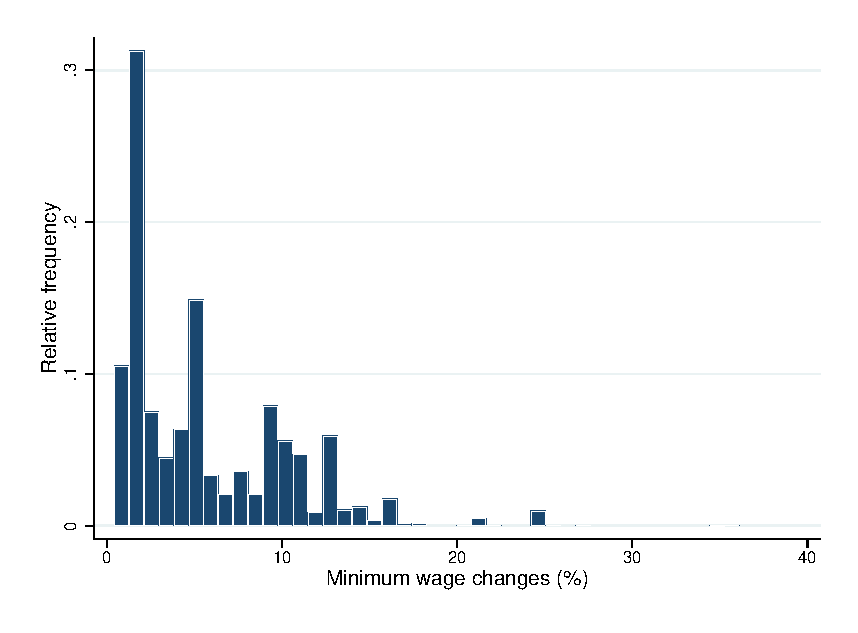
\includegraphics[width = .91\textwidth]
			{../../analysis/descriptive/output/pct_ch_mw_dist.eps}
		\end{subfigure}%
		\begin{subfigure}{.49\textwidth}
			\caption{Timing}
			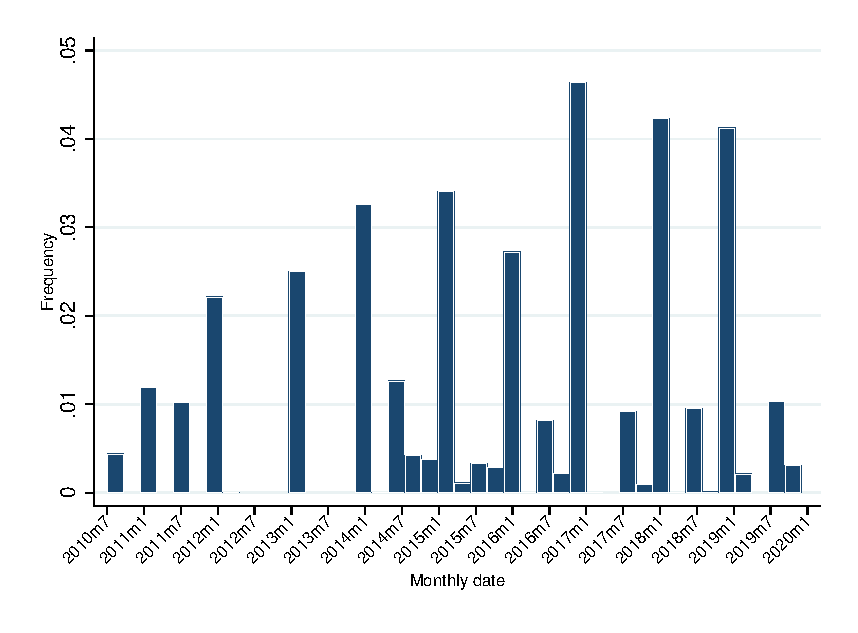
\includegraphics[width = .91\textwidth]
			{../../analysis/descriptive/output/pct_ch_mw_date_dist.eps}
		\end{subfigure}
		\begin{minipage}{.95\textwidth} \scriptsize \vspace{1mm}
			\textit{Notes:} The histograms show the distribution of positive MW changes 
			in the full sample of ZIP codes available in the Zillow data.
		\end{minipage}
	\end{figure}
	
	\hyperlink{stat_MW}{\beamerbutton{Go Back}}
\end{frame}

\begin{frame}[label=san_diego_rents]
	\frametitle{Change in rents after CA MW Increase of January 2019 in San Diego}
	
	\hyperlink{san_diego_mw}{\beamerbutton{Go Back}}
	\vspace{-7mm}
	\begin{figure} \centering
		\includegraphics[width = .48\textwidth]
			{../../analysis/descriptive_maps/output/San_Diego_rent_msa.png}
	\end{figure}
	\vspace{-7.5mm}
	\begin{minipage}{0.95\textwidth} \scriptsize
		Notes: The figure shows the change in log median rents in Zillow between December 
		2018 and June 2019.
	\end{minipage}
\end{frame}

\begin{frame}[label = dyn_alt_model]
	\frametitle{Dynamic model: Statutory MW}
	
	Adding leads and lags of the statutory MW:
	$$
	\Delta \ln r_{ict} = \delta_t
	+ \beta \Delta \underline{w}^{\text{exp}}_{ic,t+r}
	+ \sum_{r=-s}^{s} \gamma_r \Delta \ln \underline{w}_{ict}
	+ \Delta \mathbf{X}^{'}_{ct}\eta
	+ \Delta \varepsilon_{ict}
	$$
	
	where $\{\gamma_r\}_{r=-s}^{s}$ are dynamic effects of the statutory log MW.
	
	\vspace{2mm}
	\hyperlink{dyn_model}{\beamerbutton{Go Back}}
\end{frame}

\begin{frame}[label = dyn_experienced_only]
	\frametitle{Dynamic Model: Experienced log MW Only}
	\begin{figure} \centering
		\includegraphics[width = 0.6\textwidth]
		{../../analysis/first_differences_expmw/output/dynamic_exp_only_6.eps}
	\end{figure}

	\vspace{-2mm}
	\hyperlink{dyn_stat_only}{\beamerbutton{Go Back}}
\end{frame}

\begin{frame}[label = dyn_both_alt]
	\frametitle{Dynamic Model: Experienced and Statutory MW (alternative)}
	\begin{figure} \centering
		\includegraphics[width = 0.6\textwidth]
		{../../analysis/first_differences_expmw/output/dynamic_exp_and_statutory_inv_6.eps}
	\end{figure}

	\vspace{-2mm}
	\hyperlink{dyn_both}{\beamerbutton{Go Back}}
\end{frame}

\begin{frame}[label = window_size_perturbations]
	\frametitle{Window size perturbations}
	
	\begin{columns}
		\column{0.5\textwidth}
		\begin{figure}[H]
			\centering
			\includegraphics[width = \textwidth]
			{../../analysis/first_differences_expmw/output/fd_model_comparison_expmw_3.eps}
		\end{figure}
		
		\column{0.5\textwidth}
		\begin{figure}[H]
			\centering
			\includegraphics[width = \textwidth]
			{../../analysis/first_differences_expmw/output/fd_model_comparison_expmw_9.eps}
		\end{figure}
	\end{columns}

	\hyperlink{dyn_comp}{\beamerbutton{Go Back}}
\end{frame}



\end{document}
